\documentclass[a4paper]{tufte-handout}

\usepackage{amsmath}
\usepackage{amssymb}
\usepackage{amsthm}
\usepackage{bm}
\usepackage{authblk}
\usepackage{graphicx}
\usepackage{csquotes}
\usepackage{todonotes}
\usepackage{listings}

%% color and style from arXiv:1802.02538v1 source
\definecolor{codegreen}{rgb}{0,0.6,0}
\definecolor{codegray}{rgb}{0.5,0.5,0.5}
\definecolor{codepurple}{rgb}{0.58,0,0.82}
\definecolor{backcolour}{rgb}{0.99,0.99,0.97}
\lstdefinestyle{custom}{
  language=C++,
  literate={~}{$\sim$}{1},
  backgroundcolor=\color{backcolour},   
  commentstyle=\color{codegreen},
  otherkeywords = {real, vector, matrix, data, model, parameters, transformed},
  keywordstyle=\color{magenta},
  numberstyle=\tiny\color{codegray},
  stringstyle=\color{codepurple},
  emph={		normal, cauchy, inv_gamma, bernoulli_logit, gamma	},
  emphstyle=\color{codepurple},	basicstyle={\footnotesize,\ttfamily},
  breakatwhitespace=false,         
  breaklines=true,                 
  captionpos=t,                    
  keepspaces=true,                 
  numbers=left,                    
  numbersep=5pt,                  
  showspaces=false,                
  showstringspaces=false,
  showtabs=false,                  
  tabsize=2
}
\lstdefinestyle{customInline}{
  language=C++,
  literate={~}{$\sim$}{1},
  backgroundcolor=\color{backcolour},   
  commentstyle=\color{codegreen},
  otherkeywords = {real, vector, matrix, data, model, parameters, transformed},
  keywordstyle=\color{magenta},
  stringstyle=\color{codepurple},
  emph={		normal, cauchy, inv_gamma, bernoulli_logit, gamma	},
  emphstyle=\color{codepurple},	basicstyle={\ttfamily},
  breakatwhitespace=false,         
  keepspaces=true,                 
  numbers=left,                    
  numbersep=5pt,                  
  showspaces=false,                
  showstringspaces=false,
  showtabs=false,                  
  tabsize=2
}

\renewcommand{\v}[1]{\bm{#1}}
\newcommand{\vx}{\v{x}}
\newcommand{\vt}{\v{\theta}}
\newcommand{\vb}{\v{\beta}}
\newcommand{\vm}{\v{m}}
\newcommand{\R}{\mathbb{R}}
\newcommand{\E}{\mathbb{E}}
\newcommand{\Var}{\mathbb{V}ar}
\renewcommand{\P}{\mathbb{P}}
\newcommand{\Q}{\mathbb{Q}}
\newcommand{\D}{\mathcal{D}}

\newcommand{\eq}[1]{Eq.~(\ref{eq:#1})}
\newcommand{\fig}[1]{Fig.~\ref{fig:#1}}

\newtheorem{definition}{Definition}
\newtheorem{theorem}{Theorem}

%
% START COPYING HERE
%
\makeatletter
% Original definition of \cite from natbib package.
\DeclareRobustCommand\natcite{%
  \begingroup\let\NAT@ctype\z@\NAT@partrue\NAT@swatrue
    \@ifstar{\NAT@fulltrue\NAT@cites}{\NAT@fullfalse\NAT@cites}%
}

% Updated definition for Tufte-LaTeX
\renewcommand{\@tufte@infootnote@cite}[1]{%
  \natcite{#1}% <-- added this line
  \@tufte@add@citation{#1}%
}

% Only redefining this to get rid of a spurious space
\renewcommand\@tufte@add@citation[1]{\relax% adds a new bibkey to the list of cite keys
  \ifx\@tufte@citations\@empty\else
    \g@addto@macro\@tufte@citations{,}% separate by commas
  \fi
  \g@addto@macro\@tufte@citations{#1}% <-- stupid whitespace!
}
\makeatother
%
% STOP COPYING HERE
%

\renewcommand*{\thefootnote}{\fnsymbol{footnote}}

\title{Exploring COVID-19}

\author[1,2]{Nils Bertschinger}

\affil[1]{Frankfurt Institute for Advanced Studies, Frankfurt am Main, Germany}
\affil[2]{Goethe University, Frankfurt am Main, Germany}

\begin{document}

\maketitle%%

\renewcommand*{\thefootnote}{\Roman{footnote}}

\begin{abstract}
  The world stands still ... desperately observing the unfolding of
  the global COVID-19 pandemic.
\end{abstract}

\section{Data exploration}

The John Hopkins university and other institutes publish daily numbers
of cases and death tolls. Here, we build on their data sets and
provide some simple explorations and modeling.

\subsection{Country comparison}

\fig{rawdata} shows the raw data for several countries \footnote{Here,
  we only consider these countries in the following}.

\begin{figure}
  \begin{center}
    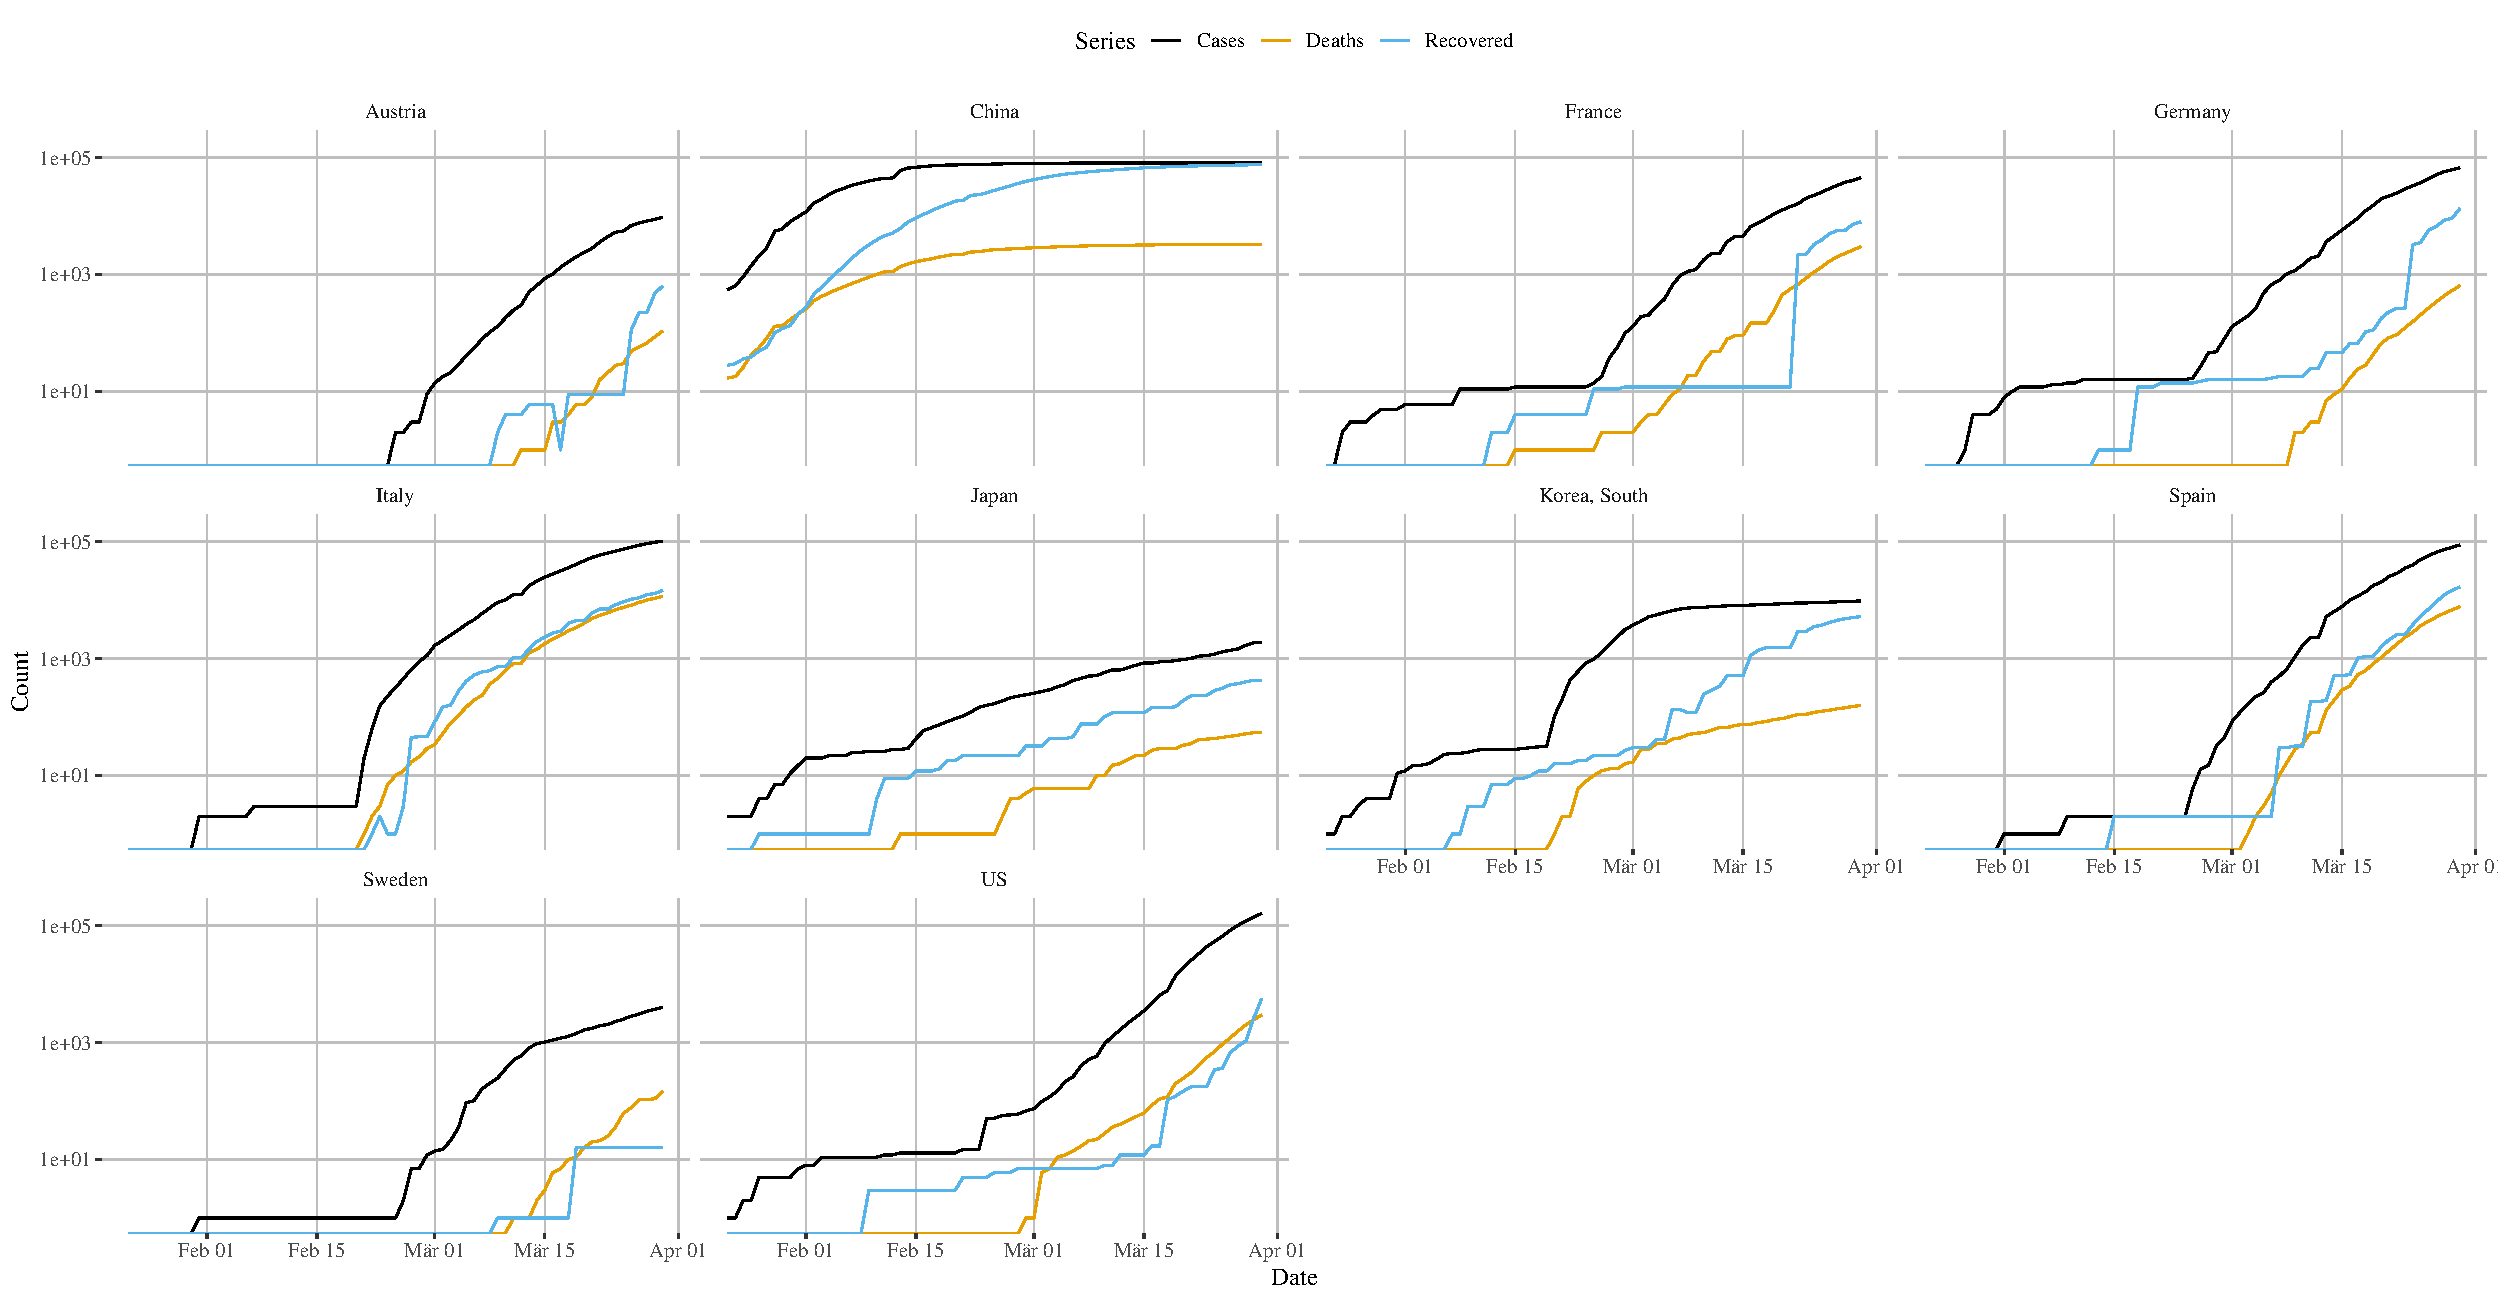
\includegraphics[width=0.95\textwidth]{figs/raw_data.pdf}
  \end{center}
  \caption{\label{fig:rawdata}Data as provided by the John Hopkins university.}
\end{figure}

As the beginning of the epidemics is different in different countries
a direct comparison is difficult. Furthermore, especially the count of
cases is highly debated and plaqued with several uncertainties. Here,
we assume that the {\em death counts are essentially reliable}. Thus,
in order to compare different countries we align all curves such that
day $0$ corresponds to the first day that either more than ten total
deaths were reported or the death rate reached a fraction of 1 per
million.

\begin{figure}
  \begin{center}
    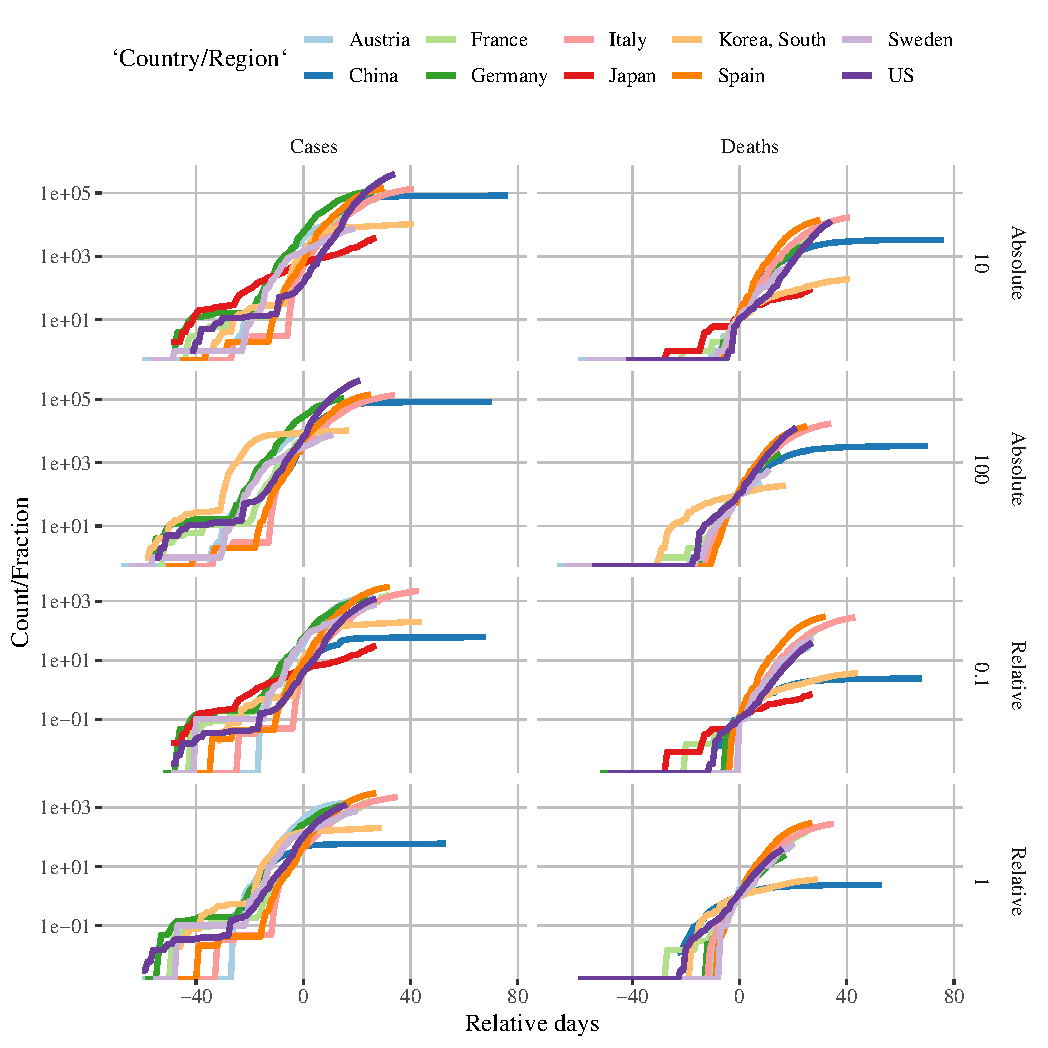
\includegraphics[width=0.95\textwidth]{figs/align_data.pdf}
  \end{center}
  \caption{\label{fig:aligndata} Case and death counts aligned to
    first day of more than 1 per million (top) or more than ten in
    total (bottom).}
\end{figure}

From the death counts in \fig{aligndata} it is evident that the
current growth rate of China, South Korea and Japan\footnote{Note that
  Japan has not yet reached 1 death per million and is thus not
  included in the upper panel.} is markedly slower than of the other
countries. Interestingly, also the case counts are somewhat aligned
even though day zero has been defined purely based on the death
counts. Furthermore, there appear to be two groups of countries with
different systematic delays between case and death counts. In
particular, Austria and Germany seem to report deaths consistently
later than France, Italy and Spain. This suggests that the
surprisingly low death rate reported for Austria and Germany could be
an artefact as reported numbers are about three to four days older
compared to other countries!

\subsection{Statistical modeling}

Indeed, it is unlikely that the death rate is very different across
different countries\footnote{There are certainly demographic and other
  aspects though.}. Next, we build a model on the assumption that the
{\em death rate is constant across all countries} and differences
purely arise from delays in reporting positively tested cases and
deaths. Overall, the model assumes the following:
\begin{itemize}
\item Case and death counts in each country grow according to a
  sigmoid function\footnote{A more realistic model should build on
    epidemic dynamics such as SEIR, but for ease of statistical
    fitting we start with sigmoid functions.} with country specific
  parameters\footnote{The basic model assumes \[ c(t) = a \frac{1}{1 +
      e^{- \beta (t - \tau)}} \; , \] i.e. a standard logistic
    function.}.
\item Observed counts are negative binomial distributed -- as an
  over-dispersed Poisson -- and delayed wrt the actual cases.
\item The probability of death is the same for all countries whereas
  the testing prevalence is country specific.
\end{itemize}

As shown in \fig{taudie}, this model\footnote{Full {\em Stan} code can
  be found in appendix \ref{app:model}.} indeed finds a consistent
difference in the delay of death counts between Austria, Germany and
France, Italy, Spain. Furthermore, the death rate -- assumed constant
across all countries -- is estimated as $3.2 \pm {1.1 \atop 0.9}
\%$. This estimate appears to be rather robust for the present model,
yet appears to be somewhat too high\footnote{Note that a naive
  estimation of the death rate, i.e. dividing contemporal case by
  death counts is biased downwards by the delay effect as actual
  deaths only realize about a week later. Accordingly the death rate
  estimate should be based on the substantially lower case counts a
  week ago. It remains to be seen if my model estimate holds up over
  time \ldots}.

Detailed model predictions for all considered countries are shown in
\fig{modelpred}. The predictions are mostly reasonable, except at the
beginning where few cases are observed and the model has difficulty of
matching the rapid leveling off observed in China and South
Korea. Interestingly, the model predicts that the curve has already
slowed markedly in Germany and Italy even though this is barely
visible in the raw numbers by now -- another example of why the delay
effect is important in understanding the dynamics of the COVID-19
pandemic.

\begin{figure}
  \begin{center}
    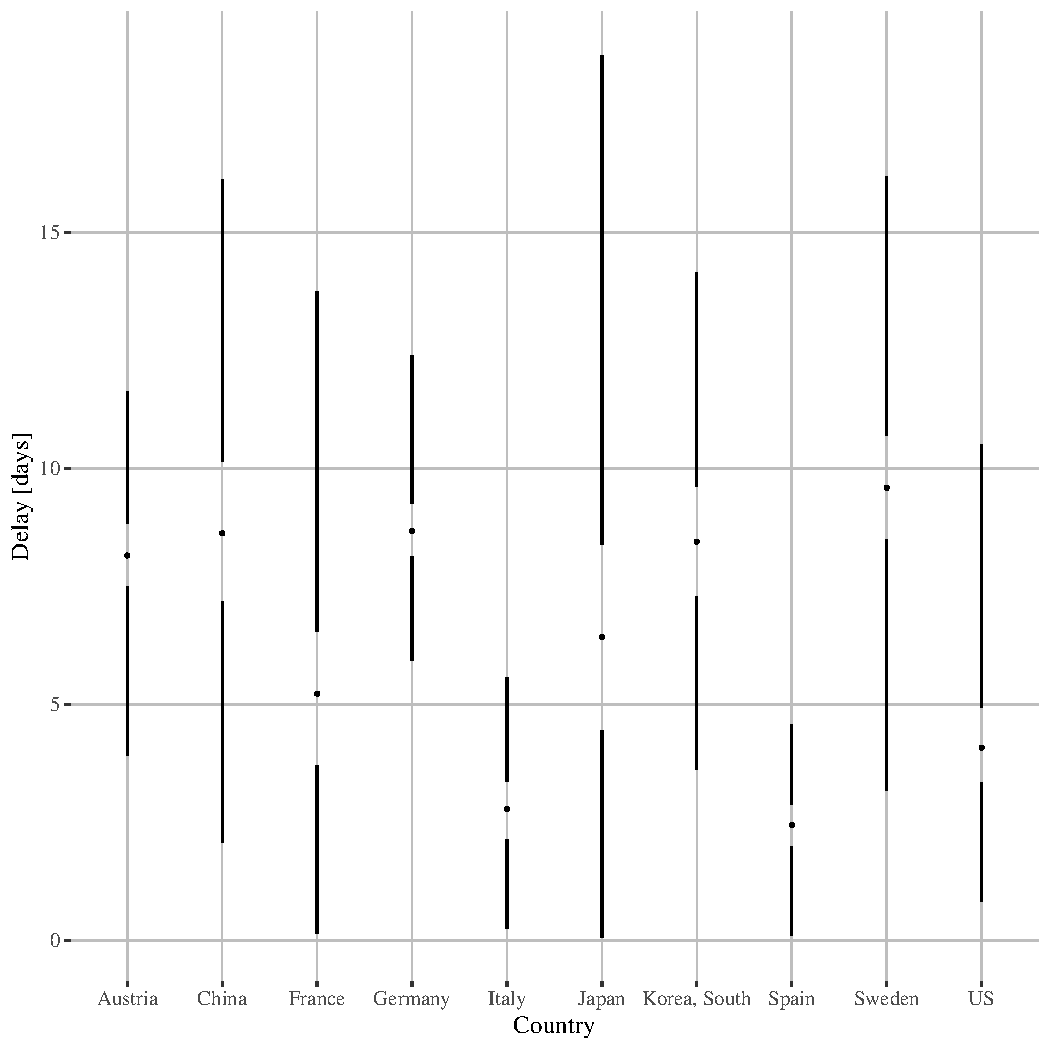
\includegraphics[width=0.95\textwidth]{figs/tau_die.pdf}
  \end{center}
  \caption{\label{fig:taudie} Model estimated delay between reported
    case and death counts.}
\end{figure}

\begin{figure*}
  \begin{center}
    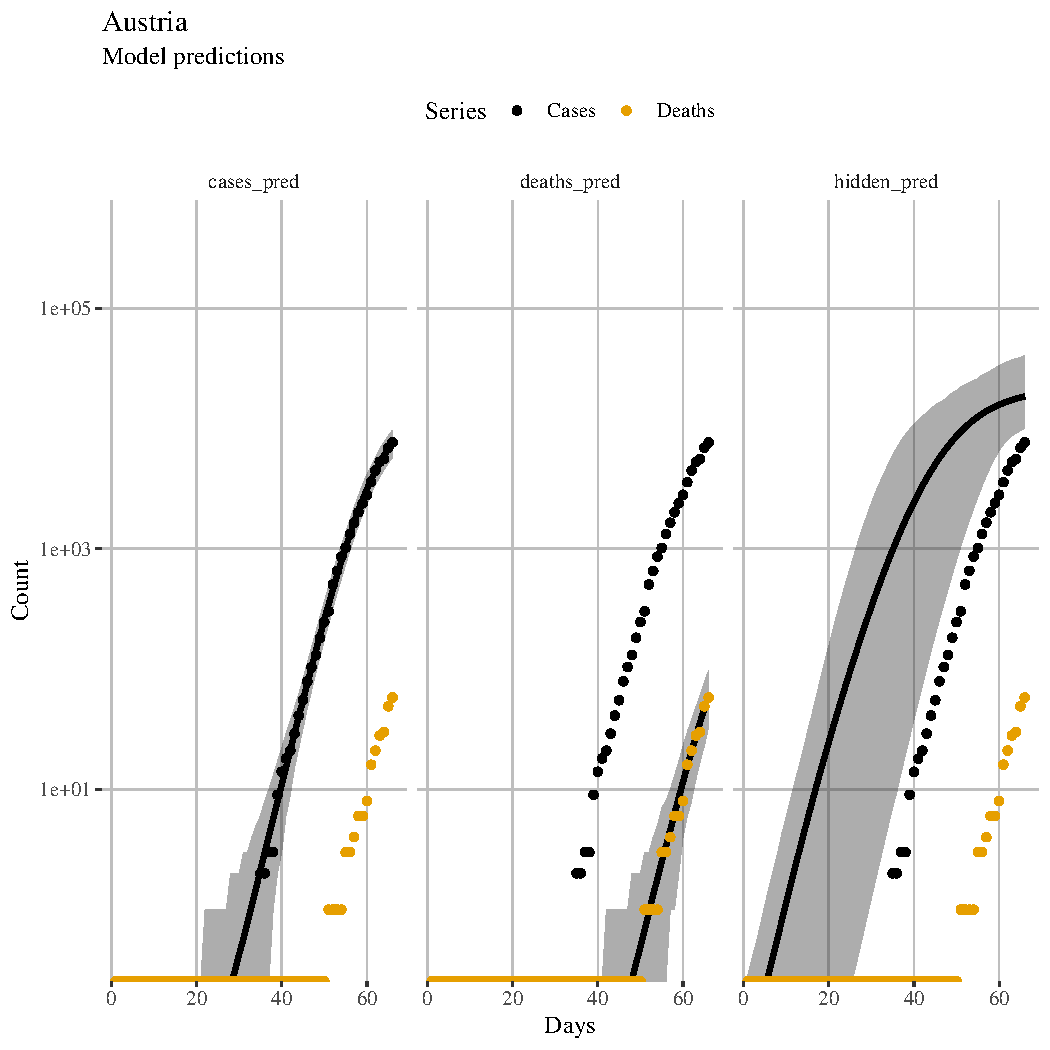
\includegraphics[width=0.45\textwidth]{figs/model_pred_AUT.pdf}
    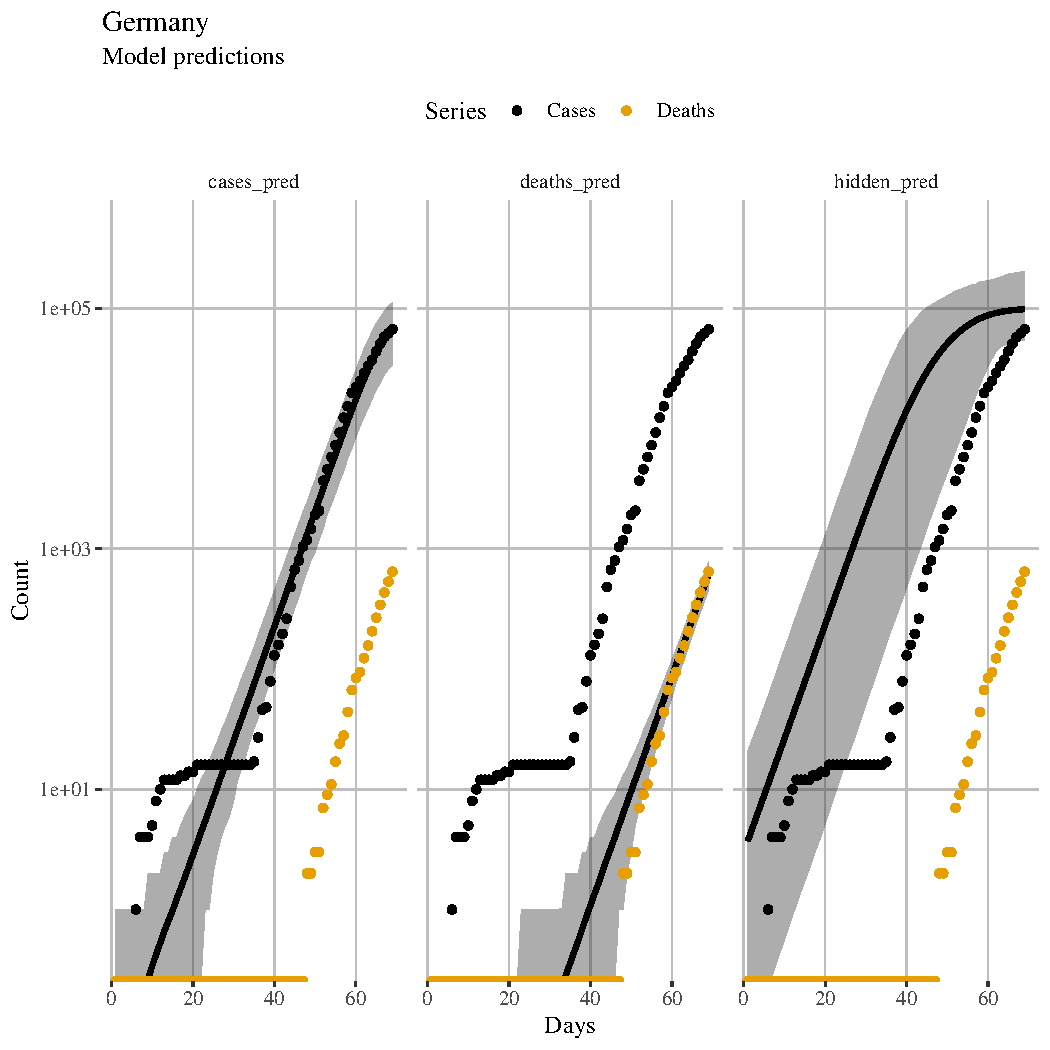
\includegraphics[width=0.45\textwidth]{figs/model_pred_DEU.pdf}
    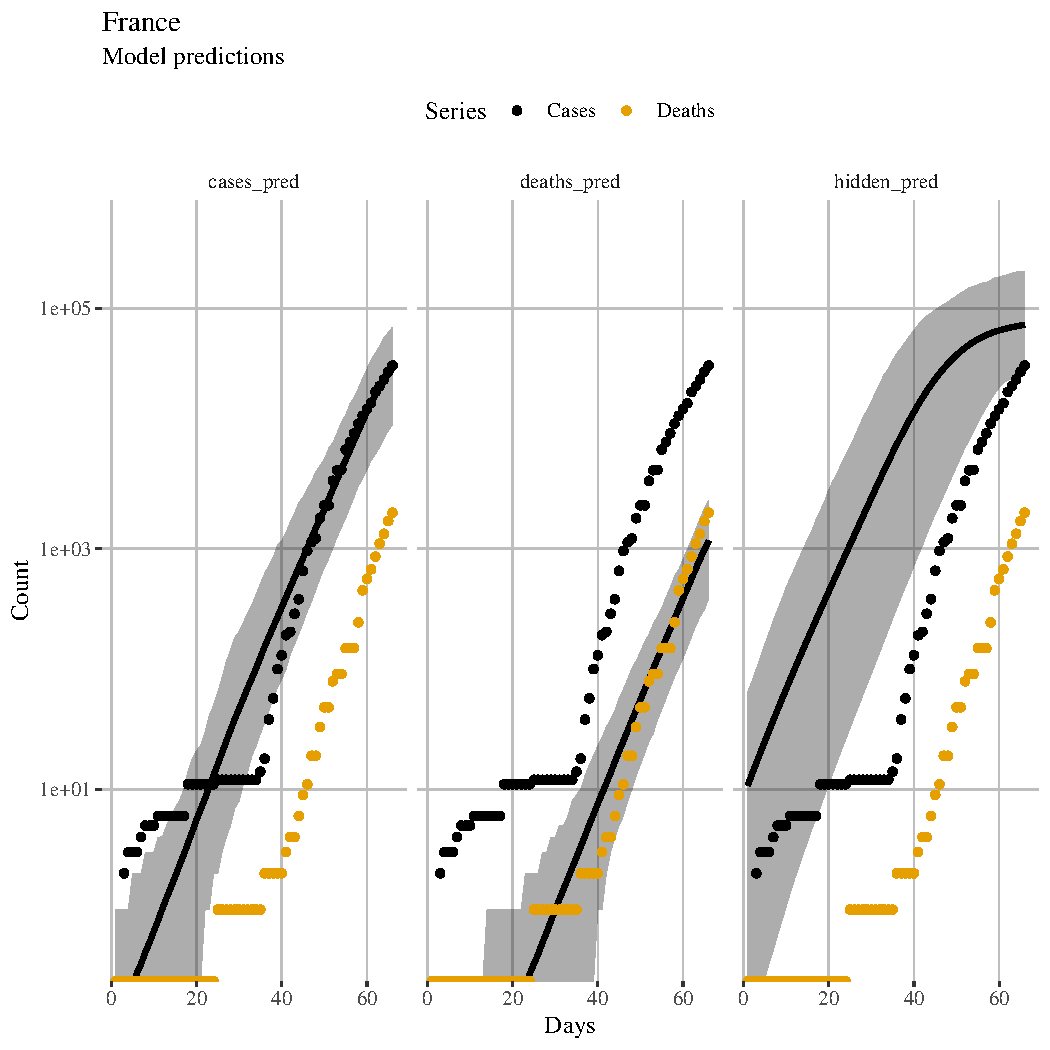
\includegraphics[width=0.45\textwidth]{figs/model_pred_FRA.pdf}
    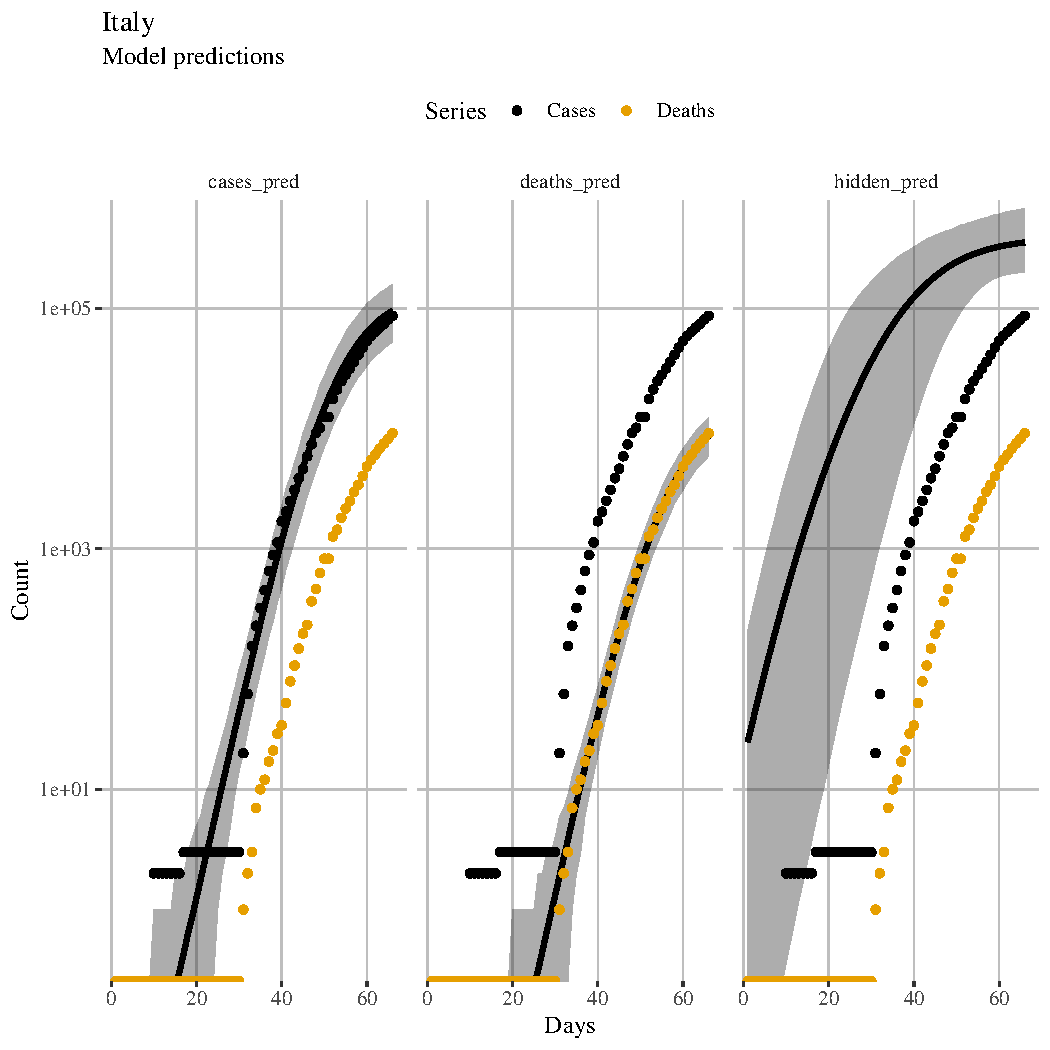
\includegraphics[width=0.45\textwidth]{figs/model_pred_ITA.pdf}
    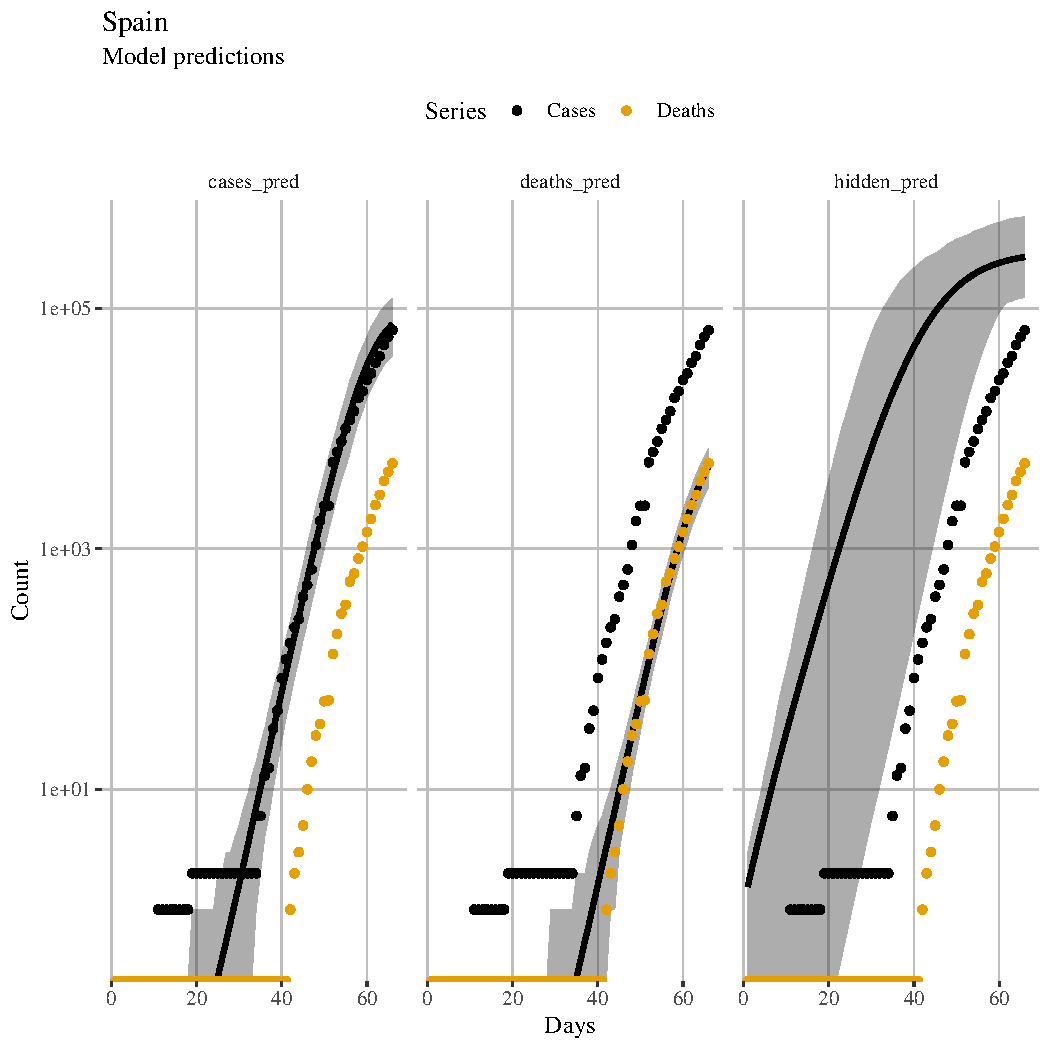
\includegraphics[width=0.45\textwidth]{figs/model_pred_ESP.pdf}
    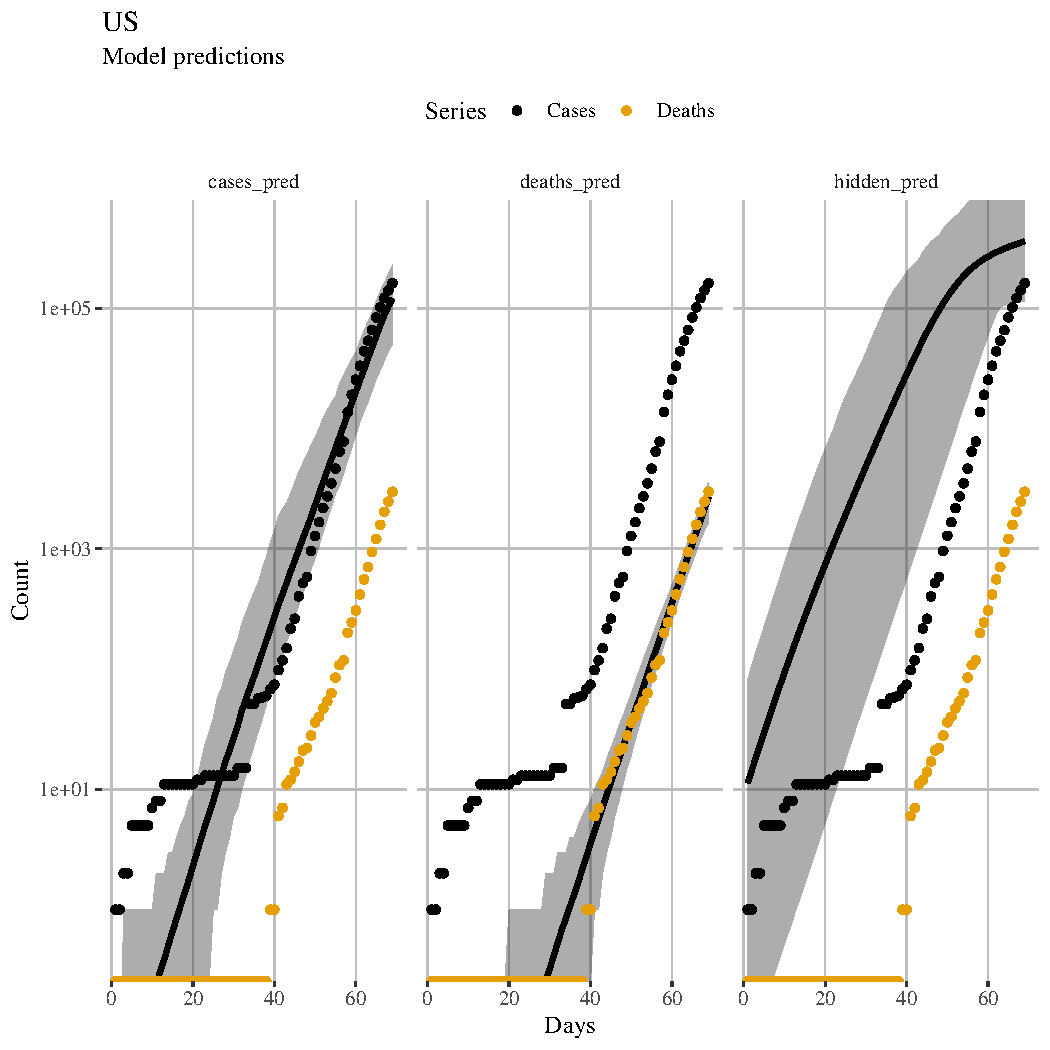
\includegraphics[width=0.45\textwidth]{figs/model_pred_USA.pdf}
    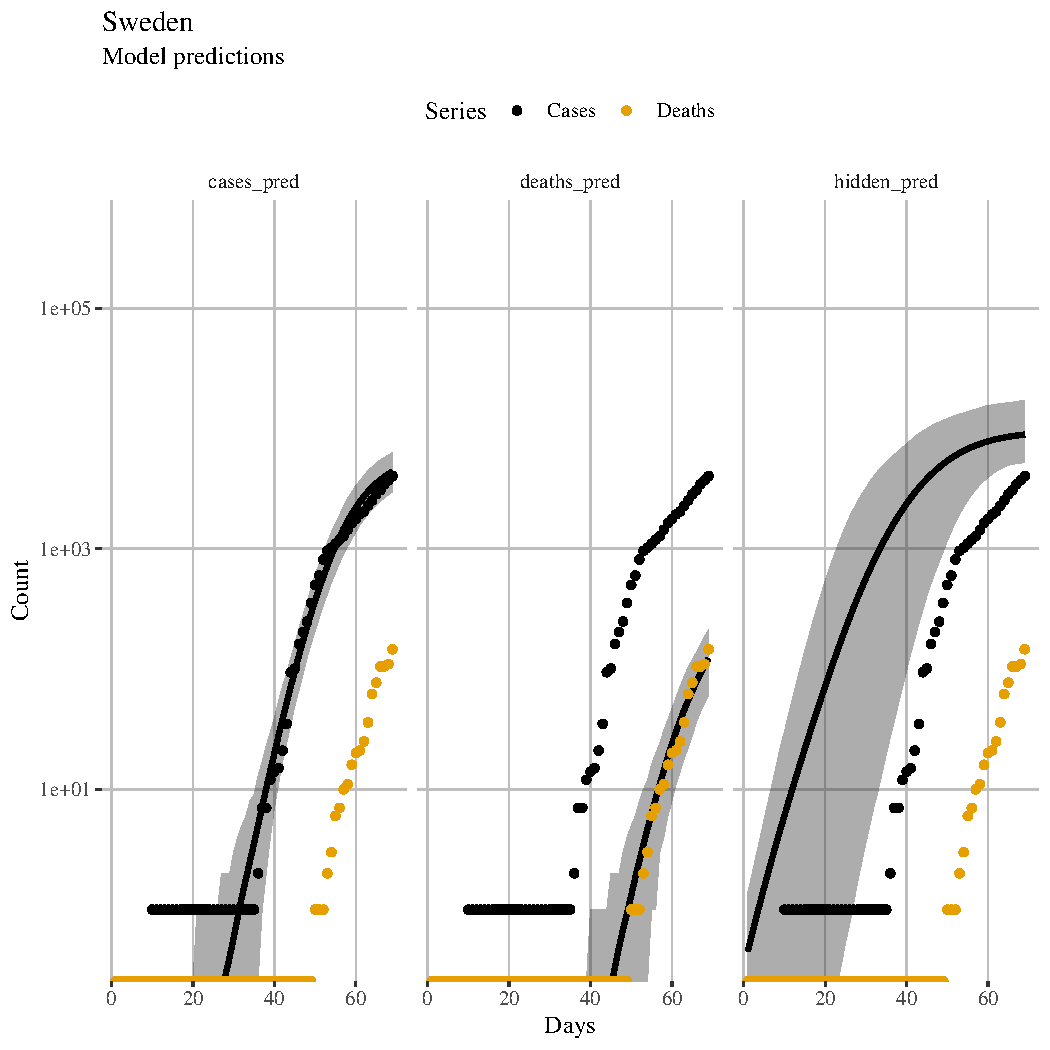
\includegraphics[width=0.45\textwidth]{figs/model_pred_SWE.pdf}
    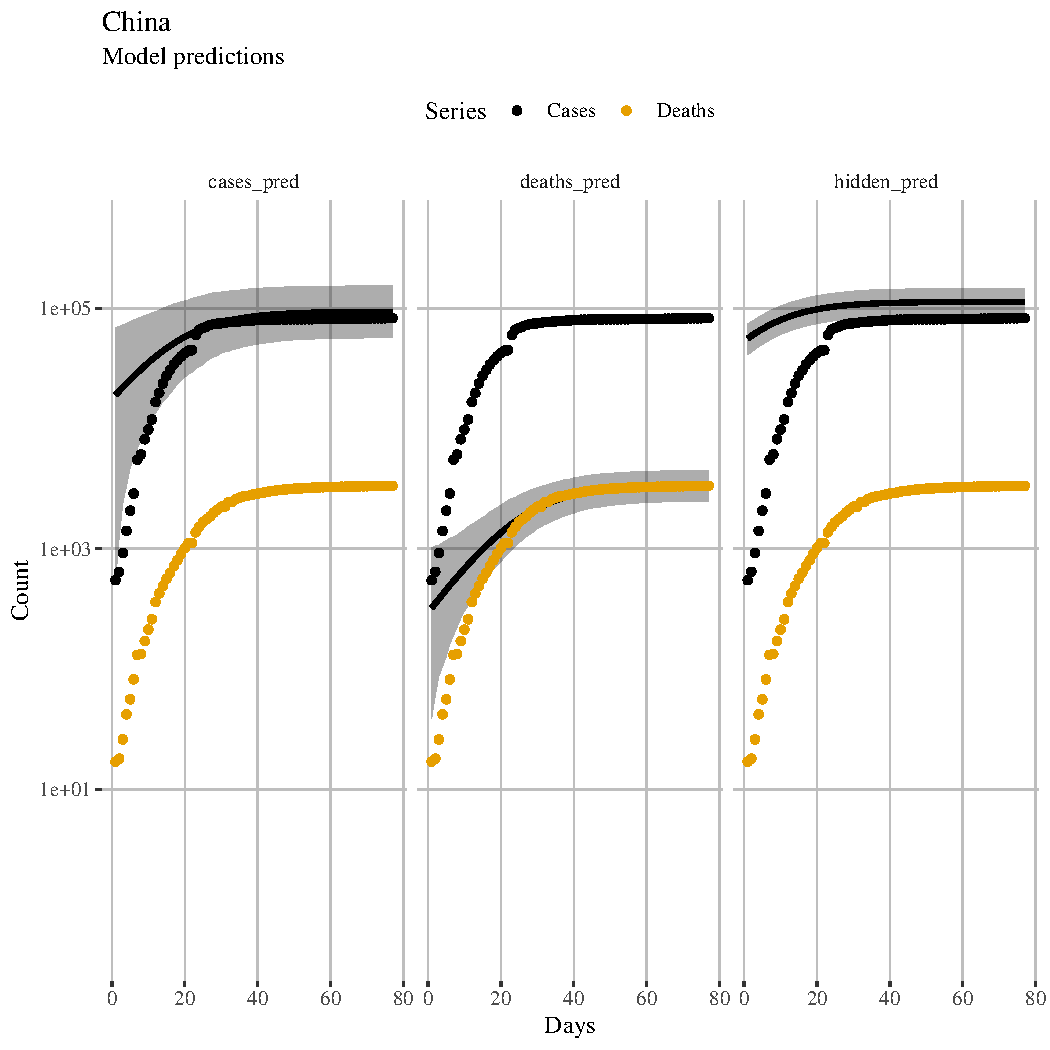
\includegraphics[width=0.45\textwidth]{figs/model_pred_CHN.pdf}
    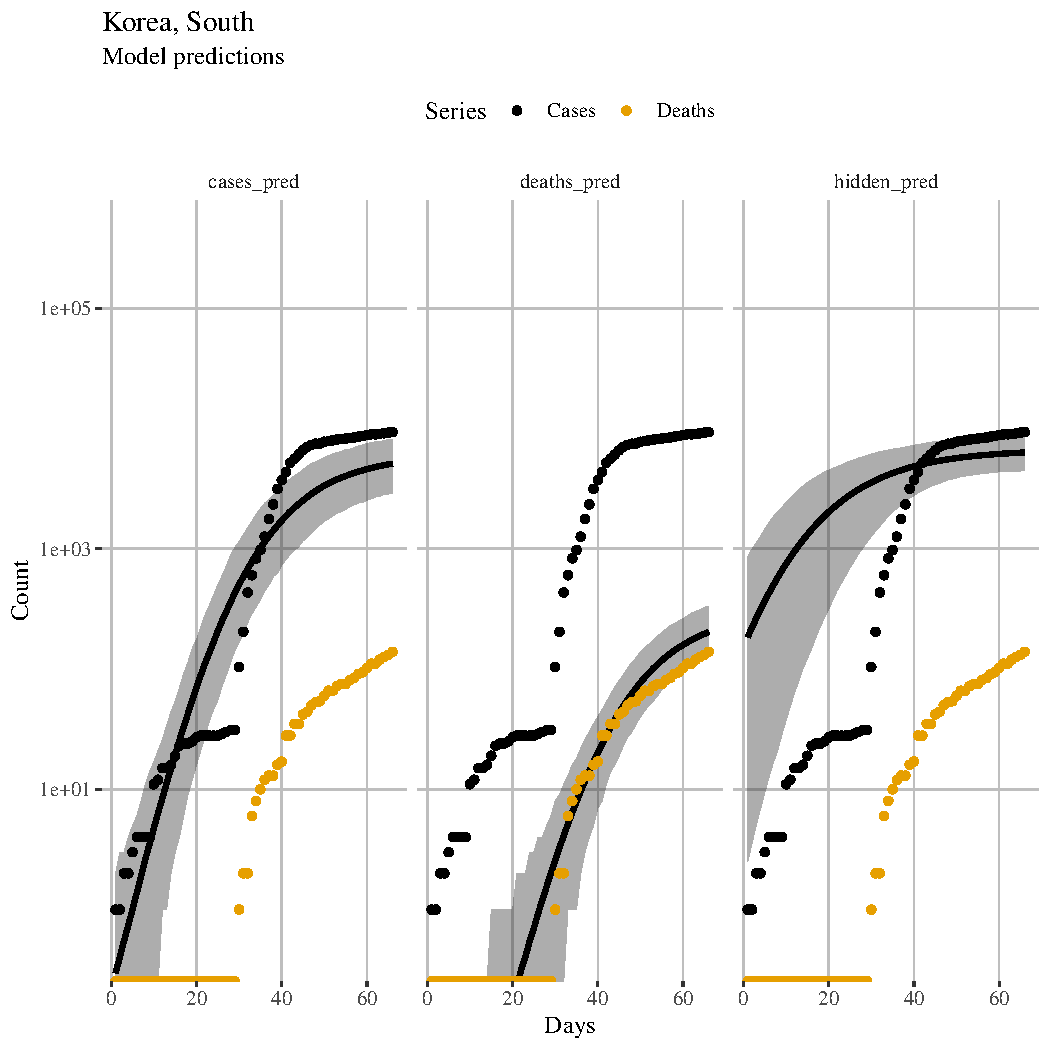
\includegraphics[width=0.45\textwidth]{figs/model_pred_KOR.pdf}
    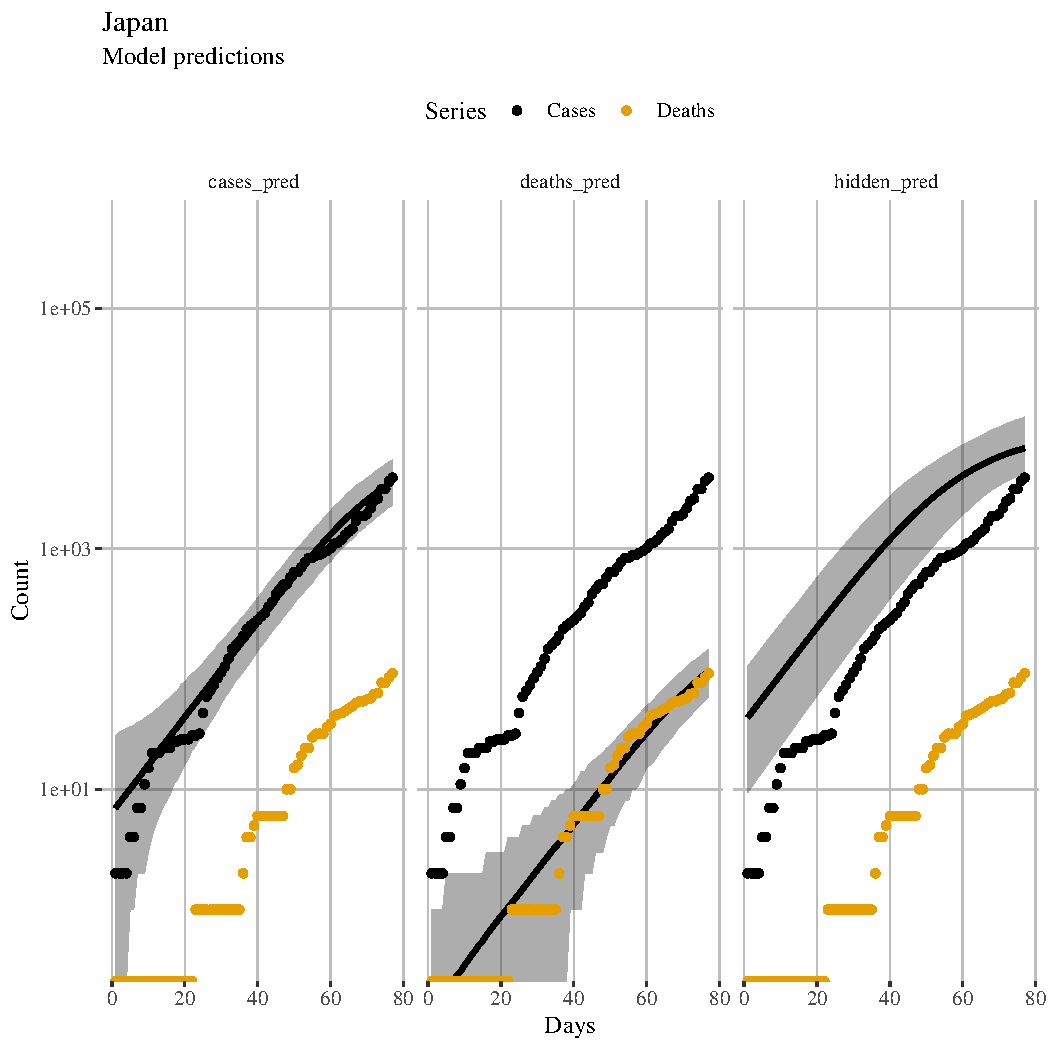
\includegraphics[width=0.45\textwidth]{figs/model_pred_JPN.pdf}
  \end{center}
  \caption{\label{fig:modelpred} Model predictions (mean and 95\%
    credible region) of actual (hidden) and observed case and death
    counts for different countries.}
\end{figure*}

\section{Financial markets}

\subsection{Implied risk-neutral densities}

\begin{marginfigure}
  \begin{center}
    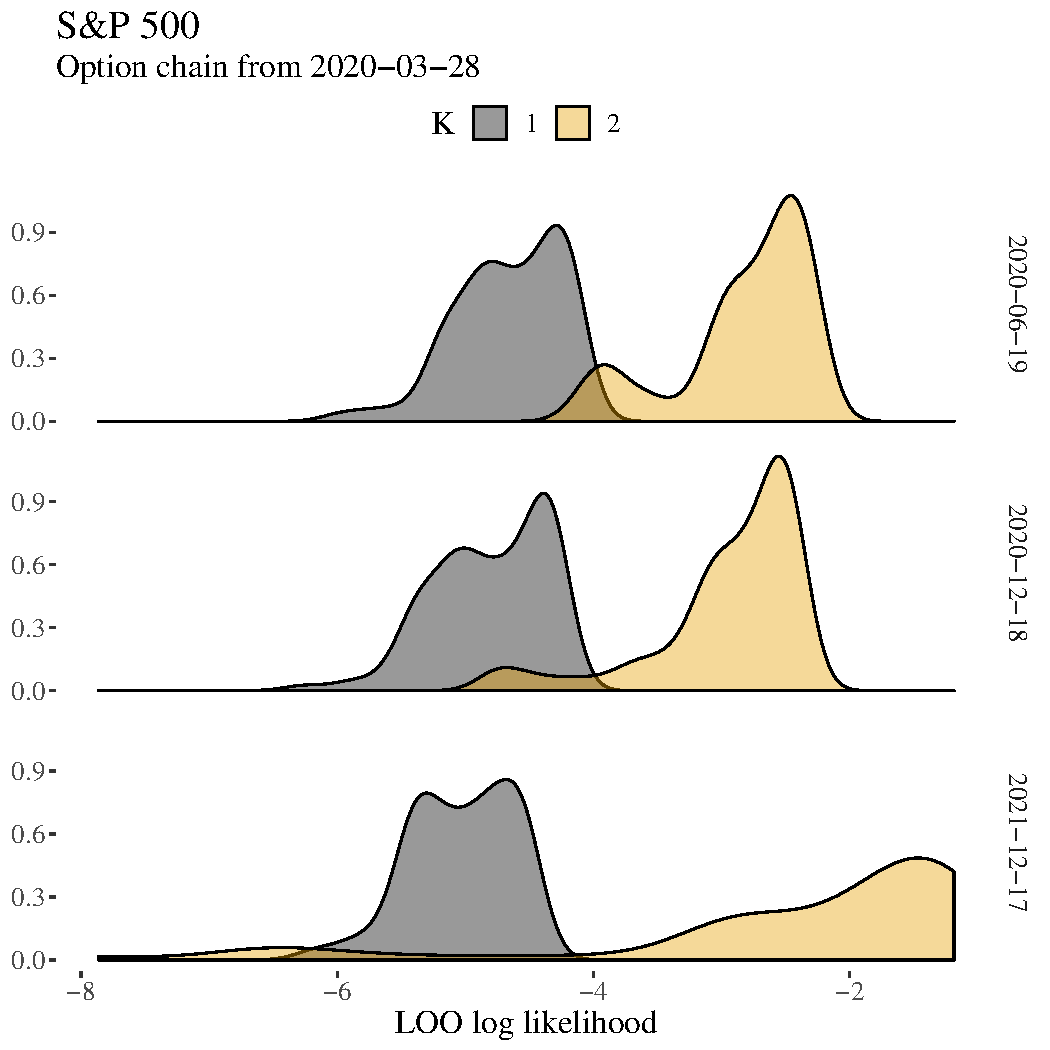
\includegraphics[width=0.95\textwidth]{model_loo.pdf}
  \end{center}
  \caption{Visual model comparison based on LOO log likelihood.}
\end{marginfigure}

\begin{figure}
  \begin{center}
    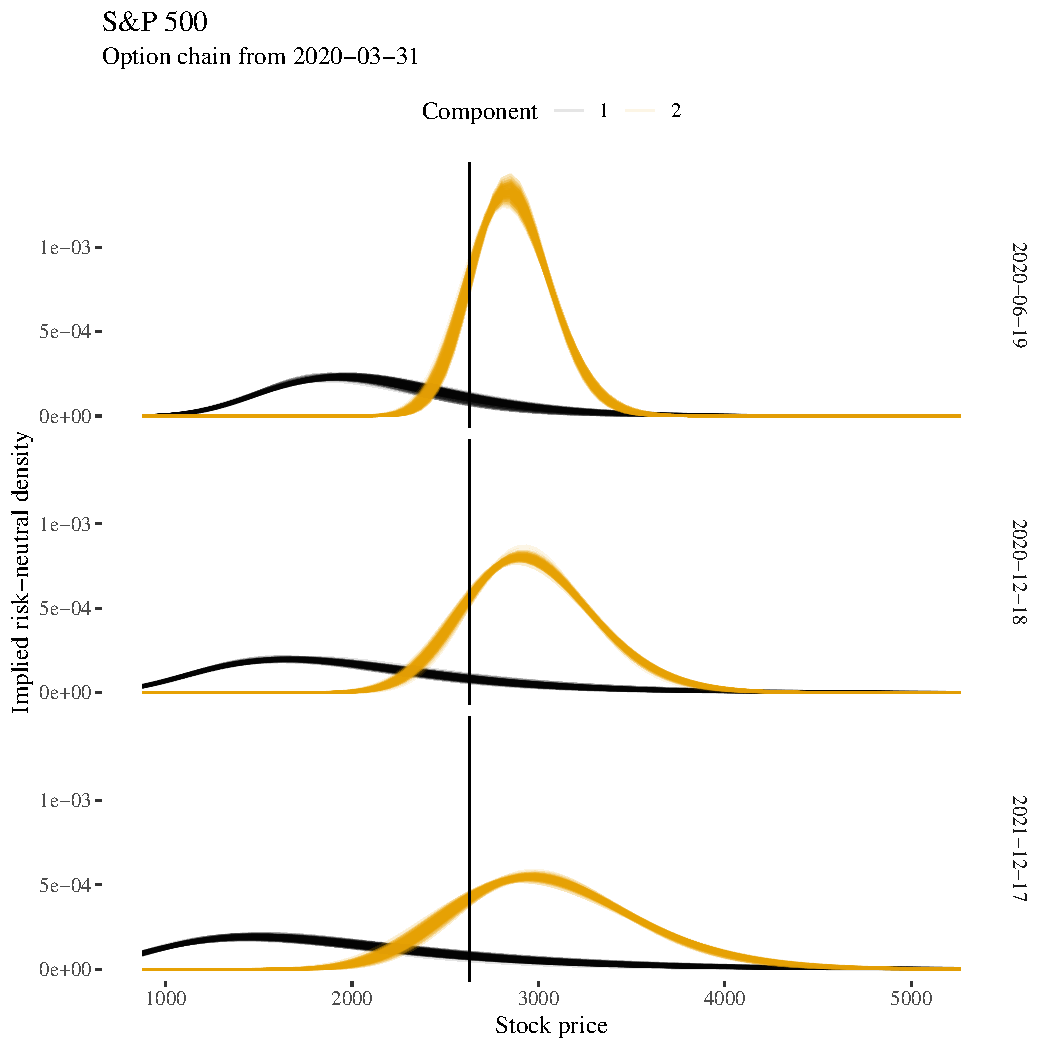
\includegraphics[width=0.95\textwidth]{risk_neutral.pdf}
  \end{center}
  \caption{Components of fitted implied risk-neutral density. Shown
    are 100 draws from the posterior distribution.}
\end{figure}

\begin{marginfigure}
  \begin{center}
    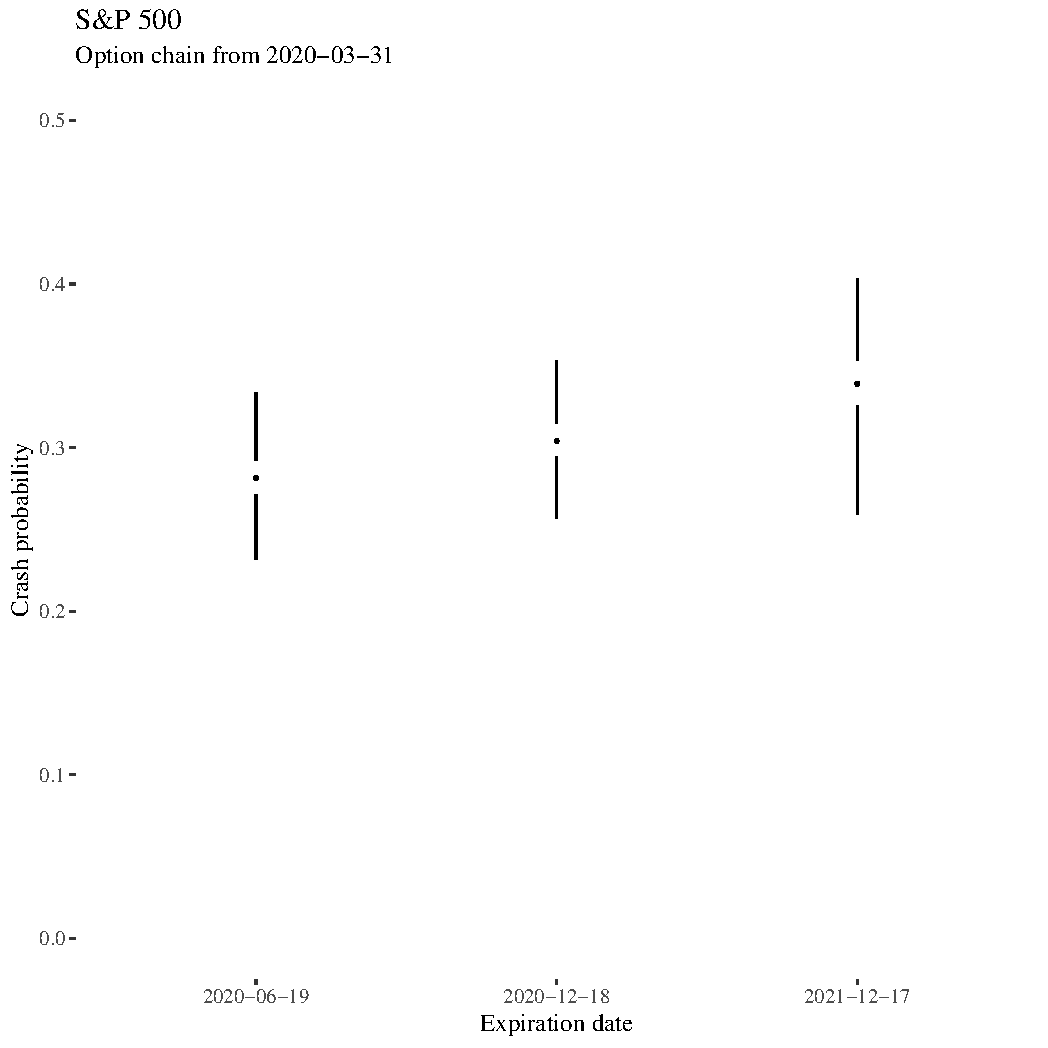
\includegraphics[width=0.95\textwidth]{crash_prob.pdf}
  \end{center}
  \caption{Market implied crash probability derived from two component
    mixture model.}
\end{marginfigure}

\appendix

\section{Sigmoid model code}
\label{app:model}
\lstinputlisting[style=custom,firstline=1]{../growth.stan}

\end{document}
